\section*{Introduction}

\begin{frame}{Introduction}
    You have an awesome algorithm, \textbf{but}:
    
    \begin{center}
        \color{blue} How can you ensure that it behaves better \wrt{} state-of-the-art?
    \end{center}

    \begin{itemize}
        \item Theoretically? What if it's too complex?
        \item By comparing its \textit{performances} on different \textit{scenarios} with different \textit{state-of-the-art algorithms}? 
    \end{itemize}

    $$\Downarrow$$

    \textbf{Problem:} the scenarios and the comparing algorithms may lead to too many combinations!
    
    \textbf{Goal:} design a extensible framework that automatically performs all the combinations required for your performance testing;

    \textbf{Result} a new Python software called \code{phd-tester} which performs automatic testing. Code available at \textsc{https://github.com/Koldar/phdTester} 
\end{frame}

\begin{frame}{A Motivating Example (1)}
    \textbf{Context:} \textit{dynamic} single agent pathfinding (given a weighted directed graph $\mathcal{G} = \langle N, E\rangle$, a \textit{start} vertex $s$, a \textit{goal} vertex $t$, what is the optimal path allowing an agent to reach $t$ from $s$?);

    \textit{dynamic} in the sense that, at the beginning of each pathfinding, some (arbitrary) edges temporary increase their cost (\textit{perturbations}).

    \textbf{Example}: going from $s = n_1$ to $t = n_5$
    \begin{figure}[ht]
        \centering
        \begin{subfigure}{0.45\linewidth}
            \centering
            \begin{tikzpicture}
                \tikzset{Node/.style={circle, thick, draw=blue!80, fill=blue!40, minimum size=0.5cm}}
                \tikzset{OptimalPath/.style={circle, thick, draw=blue!80, fill=blue!40, minimum size=0.5cm}}
        
                \node[Node](N01) at (1.5,5) {$n_{1}$};
                \node[Node](N02) at (2,3.5) {$n_{2}$};
                \node[Node](N03) at (3,6.5) {$n_{3}$};
                \node[Node](N04) at (4,3.6) {$n_{4}$};
                \node[Node](N05) at (4,5.5) {$n_{5}$};
        
                \draw[-{Latex[length=2mm,width=3mm]}]
                    (N01) edge node[above=1mm,xshift=-3pt]{$1$} (N03) 
                    (N03) edge node[above=1mm]{$8$} (N05)
                    (N01) edge node[right=1mm]{$2$} (N02) 
                    (N04) edge node[pos=0.2,left=1mm]{$2$} (N05)
                    (N02) edge node[pos=0.4,above=1mm]{$3$} (N04)
                ;

                \draw[-{Latex[length=2mm,width=3mm]}, line width=1mm]
                    (N01) edge node[above=1mm]{$6$} (N05) 
                ;
            \end{tikzpicture}
            \caption{original graph}
            \label{fig:pathfinding:idea:single edgecostschanges:a}
        \end{subfigure}\quad%
        \begin{subfigure}{0.45\linewidth}
            \centering
            \begin{tikzpicture}
                \tikzset{Node/.style={circle, thick, draw=blue!80, fill=blue!40, minimum size=0.5cm}}
                \tikzset{OptimalPath/.style={circle, thick, draw=blue!80, fill=blue!40, minimum size=0.5cm}}
        
                \node[Node](N01) at (1.5,5) {$n_{1}$};
                \node[Node](N02) at (2,3.5) {$n_{2}$};
                \node[Node](N03) at (3,6.5) {$n_{3}$};
                \node[Node](N04) at (4,3.6) {$n_{4}$};
                \node[Node](N05) at (4,5.5) {$n_{5}$};
        
                \draw[-{Latex[length=2mm,width=3mm]}]
                    (N01) edge node[above=2mm,xshift=-3pt]{{\color{red} $\xcancel{1}$} $2$} (N03) 
                    (N03) edge node[above=1mm]{$8$} (N05)
                    (N01) edge node[above=1mm]{{\color{red} $\xcancel{6}$} $11$} (N05) 
                ;

                \draw[-{Latex[length=2mm,width=3mm]}, line width=1mm]
                    (N01) edge node[right=1mm]{$2$} (N02) 
                    (N02) edge node[pos=0.4,above=1mm]{{\color{red} $\xcancel{3}$} $5$} (N04)
                    (N04) edge node[pos=0.2,left=1mm]{$2$} (N05)
                ;
            \end{tikzpicture}
            \caption{Graph temporary altered}
            \label{fig:pathfinding:idea:single edgecostschanges:b}
        \end{subfigure}%
    \end{figure}
\end{frame}

\begin{frame}{A Motivating Example (2)}
    We can solve it:
    \begin{itemize}
        \item 4 Algorithms: Dijkstra, \code{ALT}, A* + Euclidean Distance, A* + CPD, \textbf{CPD search} (our technique!);
        \item On which map? hrt201, dustwallowkeys, mazes512-1-4, rooms16-003, ...;
        \item How to generate perturbations? \textbf{R}andomly? If so how many \textbf{E}dges should we affect? Or by affecting a specific \textbf{A}rea along the optimal path? If so, how \textbf{W}ide the area is? Where should we affect the \textbf{P}ath?
    \end{itemize}
\end{frame}

\begin{frame}{A Motivating Example (3)}
    \begin{figure}
        \centering
        \begin{subfigure}{0.49\textwidth}
            \begin{tikzpicture}
                \tikzstyle{vertex} = [shape=rectangle, rounded corners=1mm, draw=blue!50, fill=blue!20, thick, minimum size=3mm, inner sep=3pt, node distance=1.0cm and 0.1cm];
                \tikzstyle{vertex2} = [shape=rectangle, rounded corners=1mm, draw=red!50, fill=red!20, thick, minimum size=3mm, inner sep=3pt, node distance=1cm and 0.1cm];
    
                \node[vertex](Algorithms) at (0,0) {Algorithms};
                \node[vertex, below =of Algorithms](Dijkstra) {Dijkstra};
                \node[vertex, left =of Dijkstra](ALT) {ALT};
                \node[vertex, right =of Dijkstra](Astar) {A*};
                \node[vertex, right =of Astar](CPDSearch) {CPDSearch};
                \node[vertex2, below left =of Astar](Euclidean) {Euclidean};
                \node[vertex2, below right =of Astar](CPD) {CPD};
    
                \draw[-{Latex[length=2mm,width=3mm]}, line width=1mm]
                    (Algorithms) edge node[]{} (Dijkstra) 
                    (Algorithms) edge node[]{} (ALT) 
                    (Algorithms) edge node[]{} (Astar) 
                    (Algorithms) edge node[]{} (CPDSearch)
                    (Astar) edge node[]{} (Euclidean)  
                    (Astar) edge node[]{} (CPD) 
                ;
            \end{tikzpicture}
        \end{subfigure}\hfill%
        \begin{subfigure}{0.49\textwidth}
            \begin{tikzpicture}
                \tikzstyle{vertex} = [shape=rectangle, rounded corners=1mm, draw=blue!50, fill=blue!20, thick, minimum size=3mm, inner sep=3pt, node distance=1.0cm and 0.1cm];
\tikzstyle{vertex2} = [shape=rectangle, rounded corners=1mm, draw=red!50, fill=red!20, thick, minimum size=3mm, inner sep=3pt, node distance=1cm and 0.1cm];
\tikzstyle{vertex3} = [shape=rectangle, rounded corners=1mm, draw=green!50, fill=green!20, thick, minimum size=3mm, inner sep=3pt, node distance=1cm and 0.1cm];
\tikzstyle{vertex4} = [shape=rectangle, rounded corners=1mm, draw=yellow!50, fill=yellow!20, thick, minimum size=3mm, inner sep=3pt, node distance=1cm and 0.1cm];
\tikzstyle{vertex5} = [shape=rectangle, rounded corners=1mm, draw=cyan!50, fill=cyan!20, thick, minimum size=3mm, inner sep=3pt, node distance=1cm and 0.1cm];

\node[vertex3](Maps) at (0,0) {Maps};
\node[vertex, right=of Maps](Perturbations) {Perturbations};
\node[vertex, below =of Perturbations](Random) {Random};
\node[vertex, left =of Random](Area) {Area};
\node[vertex2, below right =of Random](Edges) {\# Edges};
\node[vertex4, below left =of Area](Radius) {Radius};
\node[vertex5, below right=of Area](Location) {Location};

\draw[-{Latex[length=2mm,width=3mm]}, line width=1mm]
    (Perturbations) edge node[]{} (Random) 
    (Perturbations) edge node[]{} (Area) 
    (Random) edge node[]{} (Edges) 
    (Area) edge node[]{} (Radius)
    (Area) edge node[]{} (Location)  
;
            \end{tikzpicture}
        \end{subfigure}%
    \end{figure}
\end{frame}

\begin{frame}{A Motivating Example (4)}
    \begin{figure}
        \centering
        \begin{subfigure}{0.45\textwidth}
            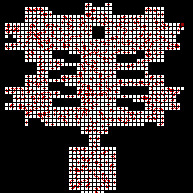
\includegraphics[width=1.0\textwidth]{{src/images/random}}
        \end{subfigure}\hfill%
        \begin{subfigure}{0.45\textwidth}
            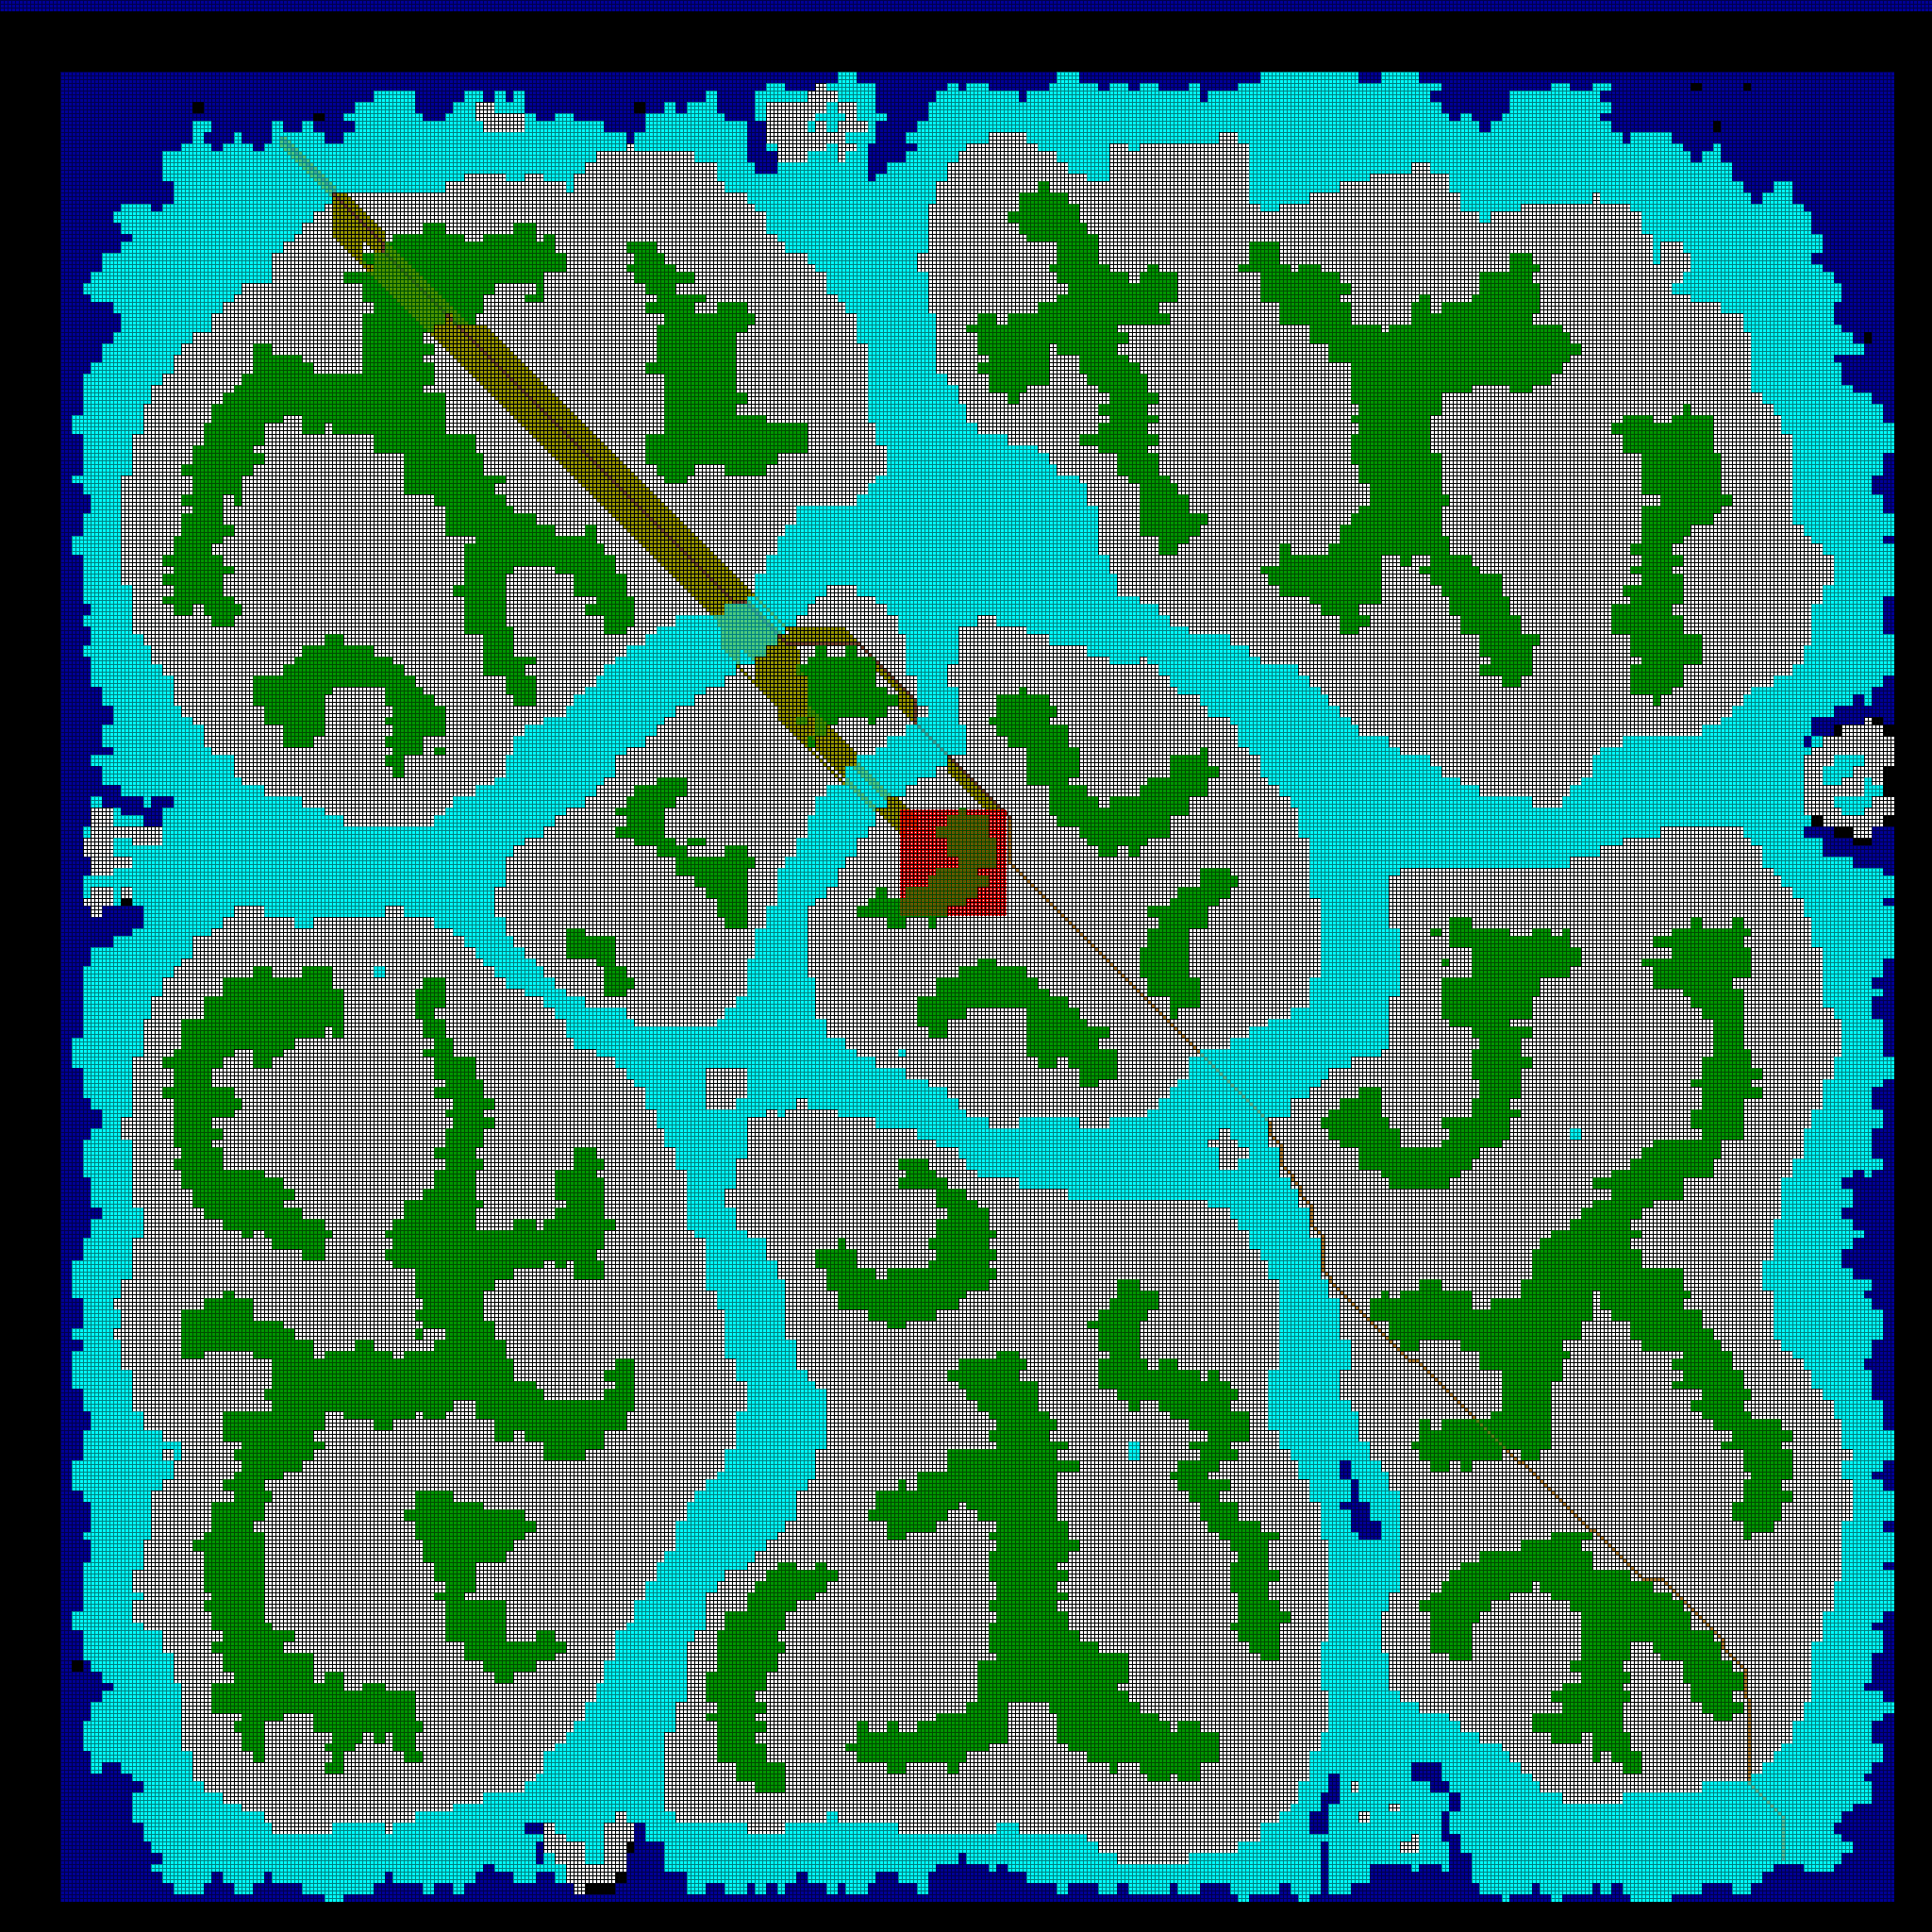
\includegraphics[width=1.0\textwidth]{{src/images/area}}
        \end{subfigure}%
        \caption{Example of perturbation policies. perturbations are shown in red. Left: random; Right: area}
    \end{figure}
\end{frame}

\begin{frame}{A Motivating Example (5)}
    $$|Algs| = 5, |Maps| = 4, |Perturbations| = 2$$ 
    $$\Downarrow$$
    $$Algs \times Maps \times Perturbations = 32$$

    But \textbf{R} depends on parameter \textbf{E} while \textbf{A} depends on \textbf{W} and \textbf{P} parameters!

    If we can choose the parameters:
    \begin{itemize}
        \item[-] $E \in \{1\%, 5\%, 10\% \}$;
        \item[-] $P \in \{20\%, 50\%, 100\% \}$;
        \item[-] $W \in \{5, 10, 15 \}$; 
    \end{itemize}
    
    Maximum combinations: $32 \cdot |E \times P \times W| = 864$!
    If we add new parameters (which, in research, it happens quite often) maximum combinations significantly increases!
\end{frame}

\begin{frame}{Talk Outline}
    The talk will be outlined as follows:
    \begin{itemize}
        \item Background: Software and design patterns used;
        \item Proposed Technique: \code{KS001}, \code{phd-tester} and the general framework flow;
        \item Conclusion and Future Works: integration with \code{CSPs} and generates automatic report pdf;
    \end{itemize}
\end{frame}